% Copyright (c) 2015 Daniele Masini - d.masini.it@gmail.com

\section{Esercizi}

\subsection{Esercizi dei singoli paragrafi}

% \begingroup
% \hypersetup{linkcolor=black}
% \subsubsection*{\ref{sect:luoghi_geometrici} - 
% \nameref{sect:luoghi_geometrici}}
% \endgroup
% 
% \begin{multicols}{2}
% 
% \end{multicols}
 
% \begingroup
% \hypersetup{linkcolor=black}
% \subsubsection*{\ref{sect:circonferenza_cerchio_def} - 
% \nameref{sect:circonferenza_cerchio_def}}
% \endgroup

\numnameref{sect:circonferenza_cerchio_def}

\begin{esercizio}
\label{ese:5.5}
Vero o falso?
\begin{enumeratea}
\item Si chiama corda il segmento che unisce il centro della 
circonferenza \\
a un suo punto\hfill\boxV\quad\boxF
\item Si chiama diametro la corda che passa per il 
centro\hfill\boxV\quad\boxF
\item Si chiama angolo alla circonferenza un angolo che ha i lati 
sulla circonferenza\hfill\boxV\quad\boxF
\item Si chiama angolo al centro un angolo che ha per vertice il 
centro \\
della circonferenza\hfill\boxV\quad\boxF
\item Due corde che si trovano alla stessa distanza dal centro sono 
congruenti\hfill\boxV\quad\boxF
\item L'angolo alla circonferenza è il doppio del corrispondente 
angolo al centro\hfill\boxV\quad\boxF
\item Una retta è esterna a una circonferenza se la sua distanza dal 
centro \\
della circonferenza è maggiore del raggio\hfill\boxV\quad\boxF
\item Due circonferenze che hanno due punti in comune si dicono 
concentriche\hfill\boxV\quad\boxF
\item Una retta che passa per il centro della circonferenza è sempre 
secante\hfill\boxV\quad\boxF
\item Una retta tangente a una circonferenza è sempre perpendicolare 
al raggio \\
che passa per il punto di tangenza\hfill\boxV\quad\boxF
\end{enumeratea}
\hfill [a)~F,\quad b)~V,\quad c)~F,\quad d)~V,\quad e)~V,\quad f)~V,\quad 
g)~V,\quad h)~F,\quad i)~V,\quad j)~V]
\end{esercizio}

\begin{multicols}{2}

\begin{esercizio}
\label{ese:5.6}
Dimostra che il luogo dei punti medi delle corde tra loro congruenti 
di una stessa circonferenza è una circonferenza.
\end{esercizio}

\begin{esercizio}
\label{ese:5.8}
Sia $OAB$ un triangolo isoscele. Si tracci la circonferenza con 
centro in $O$ e raggio $r$ minore di $OA$. Siano $C$ e $D$ i punti di 
intersezione della circonferenza con i lati obliqui del triangolo 
isoscele. Dimostra che $ABCD$ è un trapezio isoscele.
\end{esercizio}

\begin{esercizio}
\label{ese:5.9}
Siano $AB$ e $BC$ due corde congruenti di una circonferenza di centro 
$O$. Dimostra che $AO$ è bisettrice dell'angolo $B\widehat{A}C$.
\end{esercizio}


\begin{esercizio}
\label{ese:5.18}
Sia $AB$ il diametro di una circonferenza e $CD$ una corda 
perpendicolare ad $AB$. Dimostra che $ACD$ e $BCD$ sono triangoli 
isosceli.
\end{esercizio}

\begin{esercizio}
\label{ese:5.19}
Dimostra che due corde parallele e congruenti di una stessa 
circonferenza sono lati del rettangolo che ha per vertici gli estremi 
delle corde.
\end{esercizio}

% \begingroup
% \hypersetup{linkcolor=black}
% \subsubsection*{\ref{sect:proprieta_tangenti} - 
% \nameref{sect:proprieta_tangenti}}
% \endgroup

\numnameref{sect:proprieta_tangenti}

\begin{esercizio}
\label{ese:5.22}
Una retta $r$ taglia due circonferenze concentriche $C_1$ e $C_2$, 
siano $A$ e $B$ i punti individuati da $r$ sulla circonferenza $C_1$ 
e $C$ e $D$ i punti sulla circonferenza $C_2$. Dimostra che $AC$ è 
congruente a $BD$.
\end{esercizio}

\begin{esercizio}
\label{ese:5.23}
Un triangolo isoscele $ABC$ di base $BC$ è inscritto in un cerchio di 
raggio $OC$. Prolunga l'altezza $BH$ relativa al lato obliquo $AC$ 
fino a incontrare la circonferenza in $D$. Quali triangoli rettangoli 
si ottengono? Quali angoli della figura sono congruenti all'angolo in 
$D$?
\end{esercizio}

\begin{esercizio}
\label{ese:5.24}
Dimostrare che le tangenti a una circonferenza condotte dagli estremi 
di un suo diametro sono parallele tra di loro.
\end{esercizio}


\begin{esercizio}
\label{ese:5.30}
Dimostra che unendo gli estremi di due corde parallele ma non 
congruenti si ottiene un trapezio isoscele.
\end{esercizio}


\begin{esercizio}
\label{ese:5.33}
Per un punto $P$ esterno a una circonferenza di centro $O$ traccia le 
due tangenti alla circonferenza e indica con $A$ e $B$ i due punti di 
tangenza. Dimostra che la retta $PO$ è asse di $AB$. Siano $C$ e $D$ 
i punti di intersezione della retta $OP$ con la circonferenza. 
Dimostra che i triangoli $ABC$ e $ADB$ sono isosceli. Conduci per $O$ 
il diametro parallelo alla corda $AB$, il prolungamento del diametro 
incontra le tangenti $PA$ e $PB$ rispettivamente in $E$ e in $F$. 
Dimostra che $PC$ è asse di $EF$. E che $EA$ è congruente a $BF$.
\end{esercizio}

\begin{esercizio}
\label{ese:5.34}
In una circonferenza di diametro $AB$, dagli estremi $A$ e $B$ si 
conducano due corde parallele $AC$ e $BD$. Dimostra che $AC$ è 
congruente a $BD$ e che $CD$ è un diametro.
\end{esercizio}

\begin{esercizio}
\label{ese:5.35}
In una circonferenza si disegnino due corde $AB$ e $CD$ congruenti e 
incidenti in $E$ in modo tale che $AE\cong CE$. Dimostra che gli 
estremi delle corde sono i vertici di un trapezio isoscele.
\end{esercizio}

\begin{esercizio}
\label{ese:5.36}
In una circonferenza di diametro $AB$ si individuino due punti $D$ e 
$C$ tali che siano congruenti gli angoli al centro $A\widehat{O}D$ e 
$A\widehat{O}C$. Dimostra che $BC$ è congruente a $BD$.
\end{esercizio}

\begin{esercizio}
\label{ese:5.37}
Dagli estremi della corda $AB$ di una circonferenza disegna le 
tangenti alla circonferenza stessa e sia $C$ il loro punto di 
intersezione. Dimostra che il triangolo $ABC$ è isoscele.
\end{esercizio}


\begin{esercizio}
\label{ese:5.39}
Data una circonferenza di centro $O$, da un punto $P$ tale che $PO$ 
sia congruente al diametro della circonferenza si conducano le 
tangenti alla circonferenza e siano $A$ e $B$ i punti di tangenza. 
Siano $M$ ed $N$ rispettivamente i punti medi di $PA$ e $PB$. 
Dimostra che i triangoli $ABM$ e $ABN$ sono congruenti.
\end{esercizio}

\begin{esercizio}
\label{ese:5.40}
Siano $t$ e $t'$ due tangenti ad una circonferenza negli estremi di 
un diametro $AB$. Sul prolungamento del diametro $AB$ dalla parte di 
$A$ prendi un punto $P$ e da esso conduci una tangente $t''$ alla 
circonferenza. Siano $R$ ed $S$ i punti in cui $t''$ incontra 
rispettivamente $t$ e $t'$.  Dimostra che il triangolo $ROS$ è 
rettangolo in $O$, dove $O$ è il centro della circonferenza.
\end{esercizio}

\end{multicols}

% \begingroup
% \hypersetup{linkcolor=black}
% \subsubsection*{\ref{sect:quadrilateri_circonferenza} - 
% \nameref{sect:quadrilateri_circonferenza}}
% \endgroup

\numnameref{sect:quadrilateri_circonferenza}

\begin{esercizio}
\label{ese:5.41}
Quali dei seguenti gruppi di angoli possono essere angoli interni di 
un quadrilatero inscritto in una circonferenza?
\begin{enumeratea}
\item $\alpha=80\grado$\quad$\beta=60\grado$\quad 
$\gamma=100\grado$\quad $\delta=120\grado$;
\item $\alpha=45\grado$\quad $\beta=30\grado$\quad 
$\gamma=45\grado$\quad $\delta=60\grado$;
\item $\alpha=185\grado$\quad $\beta=90\grado$\quad 
$\gamma=90\grado$\quad $\delta=15\grado$;
\item $\alpha=110\grado$\quad $\beta=120\grado$\quad 
$\gamma=70\grado$\quad $\delta=60\grado$.
\hfill [a, d]
\end{enumeratea}
\end{esercizio}

\begin{esercizio}
\label{ese:5.42}
Quali dei seguenti gruppi possono essere le lunghezze dei lati di un 
quadrilatero circoscritto ad una circonferenza?
\begin{enumeratea}
\item $a=80$ cm\quad $b=60$ cm\quad $c=\np{1000}$ cm\quad $d=120$ cm;
\item $a=\np{4,5}$ cm\quad $b=3$ cm\quad $c=\np{4,5}$ cm\quad $d=3$ cm;
\item $a=\np{18,5}$ cm\quad $b=90$ cm\quad $c=\np{0,5}$ cm\quad $d=100$cm;
\item $a=110$ cm\quad $b=120$ cm\quad $c=130$ cm\quad $d=120$ cm.
\hfill [d]
\end{enumeratea}
\end{esercizio}

\subsection{Esercizi riepilogativi}

\begin{esercizio}
\label{ese:5.43}
Di quali delle seguenti figure esiste sempre sia la circonferenza 
inscritta che quella circoscritta?
\begin{multicols}{2}
\begin{enumeratea}
\item triangolo equilatero\hfill\boxV\quad\boxF
\item triangolo isoscele\hfill\boxV\quad\boxF
\item triangolo rettangolo\hfill\boxV\quad\boxF
\item rettangolo\hfill\boxV\quad\boxF
\item rombo\hfill\boxV\quad\boxF
\item trapezio isoscele\hfill\boxV\quad\boxF
\item quadrato\hfill\boxV\quad\boxF
\item parallelogramma\hfill\boxV\quad\boxF
\item deltoide\hfill\boxV\quad\boxF
\end{enumeratea}
\end{multicols}
\hfill [a)~V,\quad b)~V,\quad c)~V,\quad d)~F,\quad e)~F,\quad f)~F,\quad 
g)~V,\quad h)~F,\quad i)~F]
\end{esercizio}

\begin{esercizio}
\label{ese:5.51}
Dimostra che in un triangolo rettangolo, la bisettrice dell'angolo 
retto è anche bisettrice dell'angolo formato dall'altezza e dalla 
mediana relative all'ipotenusa.
\end{esercizio}

\begin{esercizio}
\label{ese:5.52}
Dimostra che ogni parallelogramma circoscrivibile a una circonferenza 
è un rombo.
\end{esercizio}

\begin{esercizio}
\label{ese:5.53}
Una circonferenza di centro $O$ è inscritta in un trapezio, non 
necessariamente isoscele, di basi $AB$ e $CD$. Dimostra che gli 
angoli $A\widehat{O}D$ e $B\widehat{O}C$ sono retti.
\end{esercizio}

\begin{esercizio}
\label{ese:5.54}
Dimostra che la circonferenza inscritta e quella circoscritta a un 
quadrato sono concentriche.
\end{esercizio}

\begin{esercizio}[Prove invalsi 2003]
\label{ese:5.58}
Un esagono regolare e un quadrato hanno lo stesso perimetro. Quanto 
vale il rapporto fra un lato dell'esagono e un lato del quadrato?
\begin{multicols}{2}
\begin{enumeratea}
\item $2/3$;
\item $3/4$;
\item $1$;
\item $3/2$;
\item Dipende dal valore del perimetro.
\end{enumeratea}
\end{multicols}
\hfill [a]
\end{esercizio}

\noindent\begin{minipage}{0.7\textwidth}\parindent15pt
\begin{esercizio}[Prove invalsi 2005]
\label{ese:5.59}
Osserva la figura a lato. Quale delle seguenti affermazioni relative 
alla figura è falsa?
\begin{enumeratea}
\item Il triangolo $ABC$ è acutangolo.
\item Il punto $O$ è l'intersezione delle altezze del triangolo $ABC$.
\item Le rette $r$, $s$ e $t$ sono gli assi dei lati del triangolo 
$ABC$.
\item I punti $A$, $B$ e $C$ sono equidistanti da $O$.
\end{enumeratea}
\hfill [b]
\end{esercizio}
\end{minipage}\hfil
\begin{minipage}{0.3\textwidth}
	\centering% Copyright (c) 2015 Daniele Masini - d.masini.it@gmail.com

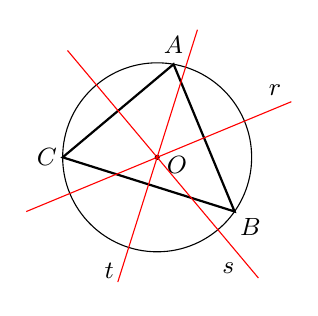
\begin{tikzpicture}[scale=0.6,font=\small]
\usetikzlibrary{calc}

\begin{scope}
%\clip (-2.1,-2.1) rectangle (2.5,2.1);
\coordinate (o) at (0,0);
\coordinate (a) at (80:2);
\coordinate (b) at (180:2);
\coordinate (c) at (325:2);

\draw (o) circle (2);

\draw[thick] (a) node[above] {$A$} -- (b) node[shift={(-0.2,0)}] {$C$} -- (c) node[shift={(0.2,-0.2)}] {$B$} -- cycle;
\draw[fill] (o) circle (1.2pt) node[shift={(0.25,-0.1)}] {$O$};
\draw[red, shorten >=-1.8cm,shorten <=-1.2cm] ($(a)!(o)!(c)$) node[black, shift={(0.9,0.6)}] {$r$} -- (o);
\draw[red, shorten >=-1.7cm,shorten <=-1.3cm] ($(b)!(o)!(c)$) node[black, shift={(-0.5,-1.1)}] {$t$} -- (o);
\draw[red, shorten >=-2cm,shorten <=-1cm] ($(a)!(o)!(b)$) node[black, shift={(1.4,-2)}] {$s$} -- (o);

\end{scope}

\end{tikzpicture}

\end{minipage}\vspace{5pt}

\noindent\begin{minipage}{0.7\textwidth}\parindent15pt
\begin{esercizio}[Prove invalsi 2007]
\label{ese:5.60}
Osserva la figura. Quale delle seguenti affermazioni è vera?
\begin{enumeratea}
\item Il triangolo è inscritto nella circonferenza minore.
\item Il triangolo è inscritto nella circonferenza maggiore.
\item La circonferenza maggiore è inscritta nel triangolo.
\item Il triangolo è circoscritto alla circonferenza maggiore.
\end{enumeratea}
\hfill [b]
\end{esercizio}
\end{minipage}\hfil
\begin{minipage}{0.3\textwidth}
	\centering% Copyright (c) 2015 Daniele Masini - d.masini.it@gmail.com

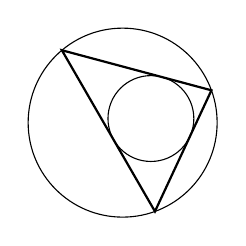
\begin{tikzpicture}[scale=0.6,font=\small]
\usetikzlibrary{calc}

\begin{scope}
\clip (-2.01,-2.01) rectangle (2.01,2.01);
\coordinate (o) at (0,0);
\coordinate (a) at (20:2);
\coordinate (b) at (130:2);
\coordinate (c) at (290:2);

\draw (o) circle (2);

\draw[thick] (a) -- (b) -- (c) -- cycle;
%\draw[fill] (o) circle (1.2pt) node[shift={(0.25,-0.1)}] {$O$};

\path (b) let \p1 = ($(a)-(b)$) in -- ($(b)!{veclen(\x1,\y1)}!(c)$) -- +($(a)-(b)$) coordinate (ob);
%\path (a) let \p1 = ($(b)-(a)$) in -- ($(a)!{-veclen(\x1,\y1)}!(c)$) -- +($(b)-(a)$) coordinate (oa);
%\coordinate (o) at (intersection of b--ob and a--oa);
\path (c) let \p1 = ($(a)-(c)$) in -- ($(c)!{veclen(\x1,\y1)}!(b)$) -- +($(a)-(c)$) coordinate (oc);
%\path (a) let \p1 = ($(c)-(a)$) in -- ($(a)!-{veclen(\x1,\y1)}!(b)$) -- +($(c)-(a)$) coordinate (ma);
%\coordinate (m) at (intersection of c--mc and a--ma);
%\coordinate (n) at (intersection of m--c and o--b);
\coordinate (oi) at (intersection of b--ob and c--oc);
\coordinate (h) at ($(b)!(oi)!(c)$);

\draw (oi) let \p1 = ($(oi)-(h)$) in circle ({veclen(\x1,\y1)});

\end{scope}

\end{tikzpicture}

\end{minipage}\vspace{5pt}

\noindent\begin{minipage}{0.65\textwidth}\parindent15pt
\begin{esercizio}[Prove invalsi 2002]
\label{ese:5.61}
Osserva la figura. I due angoli $A\widehat{C}B$ e $A\widehat{C'}B$ 
sono uguali? Quali sono le loro ampiezze in gradi?
\begin{enumeratea}
\item Non sono uguali e $A\widehat{C}B=90\grado$ e 
$A\widehat{C'}B=60\grado$
\item Non sono uguali e $A\widehat{C}B=60\grado$ e 
$A\widehat{C'}B=45\grado$
\item Sono uguali e $A\widehat{C}B=A\widehat{C'}B=60\grado$
\item Sono uguali e $A\widehat{C}B=A\widehat{C'}B=90\grado$
\item Sono uguali e $A\widehat{C}B=A\widehat{C'}B=180\grado$
\end{enumeratea}
\hfill [d]
\end{esercizio}
\end{minipage}\hfil
\begin{minipage}{0.35\textwidth}
	\centering% Copyright (c) 2015 Daniele Masini - d.masini.it@gmail.com

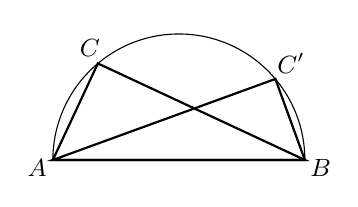
\begin{tikzpicture}[scale=0.8,font=\small]
\usetikzlibrary{calc}

\begin{scope}
\clip (-2.4,-0.3) rectangle (2.4,2.1);
\coordinate (o) at (0,0);
\coordinate (a) at (180:2);
\coordinate (b) at (0:2);
\coordinate (c) at (130:2);
\coordinate (c1) at (40:2);

\begin{scope}
\clip (-2.5,0) rectangle (2.5,2.5);
\draw (o) circle (2);
\end{scope}

\draw[thick] (a) node[shift={(-0.2,-0.1)}] {$A$} -- (b) node[shift={(0.2,-0.1)}] {$B$} -- (c) node[shift={(-0.1,0.2)}] {$C$} -- cycle;
%\draw[fill] (o) circle (1.2pt) node[shift={(0.25,-0.1)}] {$O$};
\draw[thick] (a) -- (b) -- (c1) node[shift={(0.2,0.2)}] {$C'$} -- cycle;

\end{scope}

\end{tikzpicture}

\end{minipage}\vspace{5pt}

\noindent\begin{minipage}{0.7\textwidth}\parindent15pt
\begin{esercizio}[Prove invalsi 2003]
\label{ese:5.62}
Nella figura seguente $O$ è il centro della circonferenza, $B$ un 
punto su di essa e $AC$ un suo diametro. Sapendo che 
$A\widehat{O}B=80\grado$, quanto vale $C\widehat{A}B-A\widehat{C}B$?
\begin{enumeratea}
\item $5\grado$
\item $10\grado$
\item $15\grado$
\item $20\grado$
\item $40\grado$
\end{enumeratea}
\hfill [b]
\end{esercizio}
\end{minipage}\hfil
\begin{minipage}{0.3\textwidth}
	\centering% Copyright (c) 2015 Daniele Masini - d.masini.it@gmail.com

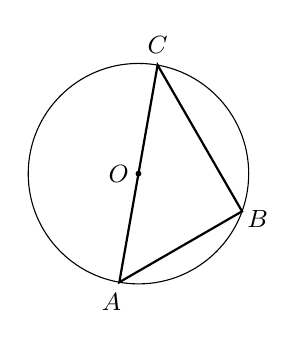
\begin{tikzpicture}[scale=0.7,font=\small]
\usetikzlibrary{calc}

\begin{scope}
%\clip (-2.1,-2.1) rectangle (2.5,2.1);
\coordinate (o) at (0,0);
\coordinate (a) at (260:2);
\coordinate (b) at (340:2);
\coordinate (c) at (80:2);

\draw (o) circle (2);

\draw[thick] (a) node[shift={(-0.1,-0.25)}] {$A$} -- (b) node[shift={(0.2,-0.1)}] {$B$} -- (c) node[shift={(0,0.25)}] {$C$} -- cycle;
\draw[fill] (o) circle (1.2pt) node[shift={(-0.25,0)}] {$O$};

\end{scope}

\end{tikzpicture}

\end{minipage}\vspace{5pt}

\begin{esercizio}[Prove invalsi 2003]
\label{ese:5.63}
Qual è il massimo numero di punti che una circonferenza e i quattro 
lati di un quadrato possono avere in comune?
\begin{multicols}{5}
\begin{enumeratea}
\item 2;
\item 4;
\item 6;
\item 8;
\item 10.
\end{enumeratea}
\end{multicols}
\hfill [d]
\end{esercizio}

\noindent\begin{minipage}{0.65\textwidth}\parindent15pt
\begin{esercizio}[Prove invalsi 2005]
\label{ese:5.64}
Osserva attentamente la figura. Sapendo che $A\widehat{O}B\cong 
C\widehat{O}D\cong B\widehat{V}C=\alpha$, quanto misura 
$A\widehat{O}D$?
\begin{multicols}{4}
\begin{enumeratea}
\item $\alpha$;
\item $2\alpha$;
\item $3\alpha$;
\item $4\alpha$.
\end{enumeratea}
\end{multicols}
\hfill [d]
\end{esercizio}
\end{minipage}\hfil
\begin{minipage}{0.35\textwidth}
	\centering% Copyright (c) 2015 Daniele Masini - d.masini.it@gmail.com

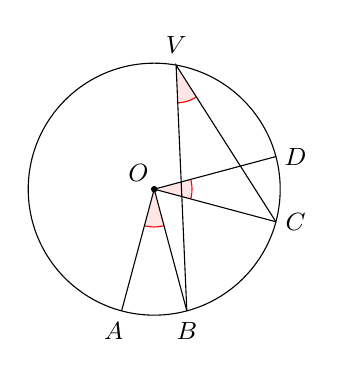
\begin{tikzpicture}[scale=0.8,font=\small]
\usetikzlibrary{calc}

\begin{scope}
%\clip (-2.1,-2.1) rectangle (2.5,2.1);
\coordinate (o) at (0,0);
\coordinate (a) at (255:2);
\coordinate (b) at (285:2);
\coordinate (c) at (-15:2);
\coordinate (d) at (15:2);
\coordinate (v) at (80:2);

\draw (o) circle (2);

\begin{scope}
\clip (a) -- (o) -- (b);
\draw[red, fill=red!10] (o) circle (0.6);
\end{scope}

\begin{scope}
\clip (c) -- (o) -- (d);
\draw[red, fill=red!10] (o) circle (0.6);
\end{scope}

\begin{scope}
\clip (b) -- (v) -- (c);
\draw[red, fill=red!10] (v) circle (0.6);
\end{scope}

\draw (a) node[shift={(-0.1,-0.25)}] {$A$} -- (o) -- (b) node[shift={(0,-0.25)}] {$B$};
\draw (c) node[shift={(0.25,0)}] {$C$} -- (o) -- (d) node[shift={(0.25,0)}] {$D$};
\draw (b) -- (v) node[shift={(0,0.25)}] {$V$} -- (c);
\draw[fill] (o) circle (1.2pt) node[shift={(-0.2,0.2)}] {$O$};

\end{scope}

\end{tikzpicture}

\end{minipage}\vspace{5pt}

\begin{esercizio}[Prove invalsi 2005]
\label{ese:5.65}
Qual è il massimo numero possibile di punti di intersezione fra una 
circonferenza e un triangolo?
\begin{multicols}{4}
\begin{enumeratea}
\item 6;
\item 5;
\item 4;
\item 3;
\end{enumeratea}
\end{multicols}
\hfill [a]
\end{esercizio}

% \newpage %-----------------------------------------------------

\begin{esercizio}[Prove invalsi 2005]
\label{ese:5.66}
Quale delle seguenti affermazioni è falsa? 
\begin{enumeratea}
\item In ogni triangolo isoscele l'altezza e la mediana relative alla 
base e la bisettrice dell'angolo al vertice coincidono.
\item In ogni triangolo isoscele baricentro, incentro, ortocentro e 
circocentro sono allineati.
\item In ogni triangolo isoscele baricentro, ortocentro, incentro e 
circocentro coincidono.
\item In ogni triangolo equilatero baricentro, ortocentro, incentro e 
circocentro coincidono.
\end{enumeratea}
\hfill [a]
\end{esercizio}

\begin{esercizio}[Prove invalsi 2006]
\label{ese:5.67}
Considera la figura seguente. Se le due circonferenze hanno raggi 
diversi, quale delle seguenti affermazioni è vera?
\begin{enumeratea}
\item Le due circonferenze sono simmetriche rispetto al punto $O$.
\item Le due circonferenze sono simmetriche rispetto a ciascuna delle 
rette $r$ e $s$.
\item $AO_1:O_2C=OC:AO$.
\item $AO_1:O_2C=AO:OC$.
\end{enumeratea}
\hfill [d]
\end{esercizio}

\begin{inaccessibleblock}[Figura: TODO]
 \begin{figure}[!htb]
	\centering% Copyright (c) 2015 Daniele Masini - d.masini.it@gmail.com

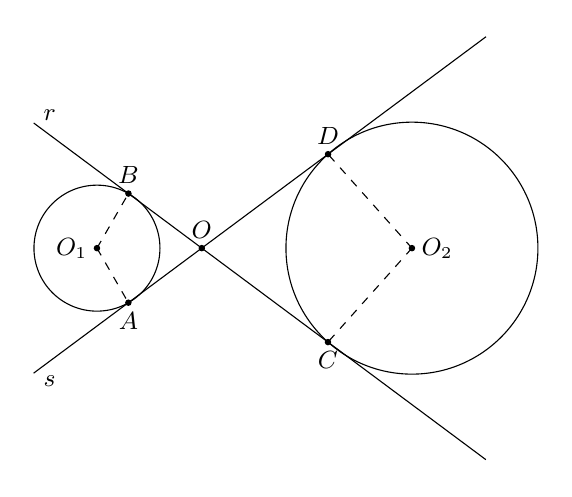
\begin{tikzpicture}[scale=0.8,font=\small]
\usetikzlibrary{calc,intersections}

\begin{scope}
\clip (-3.1,-3.5) rectangle (5.1,3.5);
\coordinate (o) at (0,0);
\coordinate (o1) at (-2,0);
\coordinate (o2) at (3,0);
\coordinate (m1) at ($(o1)!0.5!(o)$);
\coordinate (m2) at ($(o)!0.5!(o2)$);

\path[name path=Circle1] (m1) let \p1= ($(m1) - (o)$) in circle ({veclen(\x1,\y1)});
\path[name path=Circle2] (m2) let \p1= ($(m2) - (o)$) in circle ({veclen(\x1,\y1)});

\draw[name path=Circle3] (o1) circle (1);
\draw[name path=Circle4] (o2) circle (2);

\path [name intersections={of=Circle1 and Circle3}] ;
\draw[fill] (intersection-1) coordinate (b) node [above] {$B$} circle (1.2pt);
\draw[fill] (intersection-2) coordinate (a) node [below] {$A$} circle (1.2pt);
\path [name intersections={of=Circle2 and Circle4}] ;
\draw[fill] (intersection-1) coordinate (d) node [above] {$D$} circle (1.2pt);
\draw[fill] (intersection-2) coordinate (c) node [below] {$C$} circle (1.2pt);

\draw[shorten <=-1.5cm, shorten >=-2.5cm] (a) node[shift={(-1,-1)}] {$s$} -- (d);
\draw[shorten <=-1.5cm, shorten >=-2.5cm] (b) node[shift={(-1,1)}] {$r$} -- (c);

\coordinate (o3) at (intersection of a--d and b--c);

\draw[fill] (o3) circle (1.2pt) node[above] {$O$};
\draw[fill] (o1) circle (1.2pt) node[left] {$O_1$};
\draw[fill] (o2) circle (1.2pt) node[right] {$O_2$};

\draw[dashed] (o1) -- (a);
\draw[dashed] (o1) -- (b);
\draw[dashed] (o2) -- (c);
\draw[dashed] (o2) -- (d);

\end{scope}

\end{tikzpicture}

\end{figure}
\end{inaccessibleblock}

\noindent\begin{minipage}{0.65\textwidth}\parindent15pt
\begin{esercizio}
\label{ese:5.68}
Nella figura seguente il punto $O$ è il punto medio del diametro 
$AC$. L'angolo $A\widehat{O}B$ misura $40\grado$. Quanto misura 
l'angolo $O\widehat{B}C$? 
\begin{multicols}{4}
\begin{enumeratea}
\item $10\grado$;
\item $20\grado$;
\item $40\grado$;
\item $60\grado$.
\end{enumeratea}
\end{multicols}
\hfill [b]
\end{esercizio}
\end{minipage}\hfil
\begin{minipage}{0.35\textwidth}
	\centering% Copyright (c) 2015 Daniele Masini - d.masini.it@gmail.com

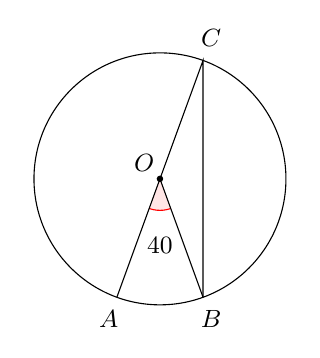
\begin{tikzpicture}[scale=0.8,font=\small]
\usetikzlibrary{calc}

\begin{scope}
\clip (-2.1,-2.4) rectangle (2.1,2.4);
\coordinate (o) at (0,0);
\coordinate (a) at (250:2);
\coordinate (b) at (290:2);
\coordinate (c) at (70:2);

\begin{scope}
\clip (a) -- (o) -- (b) -- cycle;
\draw[red, fill=red!10] (o) circle (0.5);
\node at (270:1.05) {$40\grado$};
\end{scope}

\draw[fill] (o) circle (1.2pt) node[shift={(-0.2,0.2)}] {$O$};

\draw (a) node [shift={(250:0.3)}] {$A$} -- (c) node [shift={(70:0.3)}] {$C$} -- (b) node [shift={(290:0.3)}] {$B$};
\draw (o) -- (b);

\draw (o) circle (2);

\end{scope}

\end{tikzpicture}

\end{minipage}\vspace{5pt}
